\section{Results \& Discussion}

\subsection*{Comparative Genomics Analysis}
\addcontentsline{toc}{subsubsection}{Comparative Genomics Analysis}

\normalsize

To identify genes tracing back to the last common ancestors of archaea (LACA) and bacteria (LBCA), we started from 85,205 genomes, each one the representative of species clusters, as defined by the Genome Taxonomy Database (GTDB) \cite{parks2018, parks2020, parks2022, rinke2021}. 

Genome completeness can lead to false-positive ortholog and erroneous species phylogeny inference \cite{kuzniar2008}. To ensure that phylogenetic relationships and ancestral genome reconstruction would be as accurate as possible, we filtered the genomes based on completeness and contamination cutoffs of $\geq$ 90\% and $\leq$ 5\%, respectively. This resulted in 52,614 high-quality (HQ) genomes, 1,785 archaeal and 50,829 bacterial, spanning 16 archaeal and 150 bacterial phyla. 

To evaluate the effect of taxon sampling and dataset size on ancestral gene content inference, we constructed eight genomic datasets of various sizes (16-1139 genomes). These span the phylum, class, order, family, and genus taxonomic levels for archaea, and at the phylum, class, and order taxonomic levels for bacteria. Dataset sizes can be found in table \ref{gtdb_stats_no}. Even though increasing taxon sampling has been shown to improve phylogenetic accuracy, taxon evenness markedly affects tree topology \cite{graybeal1998, martinez-gutierrez2021}. To capture, therefore, the full extant phylogenetic diversity and keep the taxon sampling even and unbiased while rendering the largest of our analyses computationally tractable, we selected a single genome for each taxon, per genomic dataset/taxonomic rank in our study.

To review the robustness of random taxon sampling we performed our analysis for three separately produced datasets both for the phylum and class taxonomic levels of archaea. Figure \ref{orthofinder_stats_figure}A shows the average percentage of genes assigned to orthogroups (OGs) for the two aforementioned triplicate runs, while \ref{orthofinder_stats_figure}C depicts the mean percentage of gene assignment in OGs for each of the archaea datasets. This statistic can act as a first-level quality control of an OrthoFinder (OF) analysis. A below 80\% mean assignment of genes in orthogroups indicates that important orthology relationships for some remaining genes are missing, likely due to poor species sampling \cite{emms2015}. Even though the number of included-in-the-analysis genomes approximately doubles per taxonomic level, the gene assignment percentage only slightly increases. The increase is justified because, as taxonomic levels become narrower, genetic distances between species decrease, allowing state-of-the-art algorithms to cluster a larger number of genes.

On a first assessment, performing a phylogenetic analysis on 51 archaea genomes (class taxonomic level) seems enough to capture the orthology relationships of protein-encoding genes. Plots \ref{orthofinder_stats_figure}A and \ref{orthofinder_stats_figure}C, however, present the average percentage of three individual OF runs, and the mean percentage of all individual species/taxa in a single OF run, respectively. They therefore conceal variance that is crucial for the analysis interpretation. To address this, we converted the percentage of genes assigned in OGs per species to a binary classification, where species with less than 80\% gene assignment were designated a "poorly sampled" status and given a value equal to zero, while the rest were given a value of one. The normalized distribution of poorly sampled taxa for each taxonomic level analysis can be seen in Figure \ref{orthofinder_stats_figure}D.

\begin{figure}[H]
    \centering
    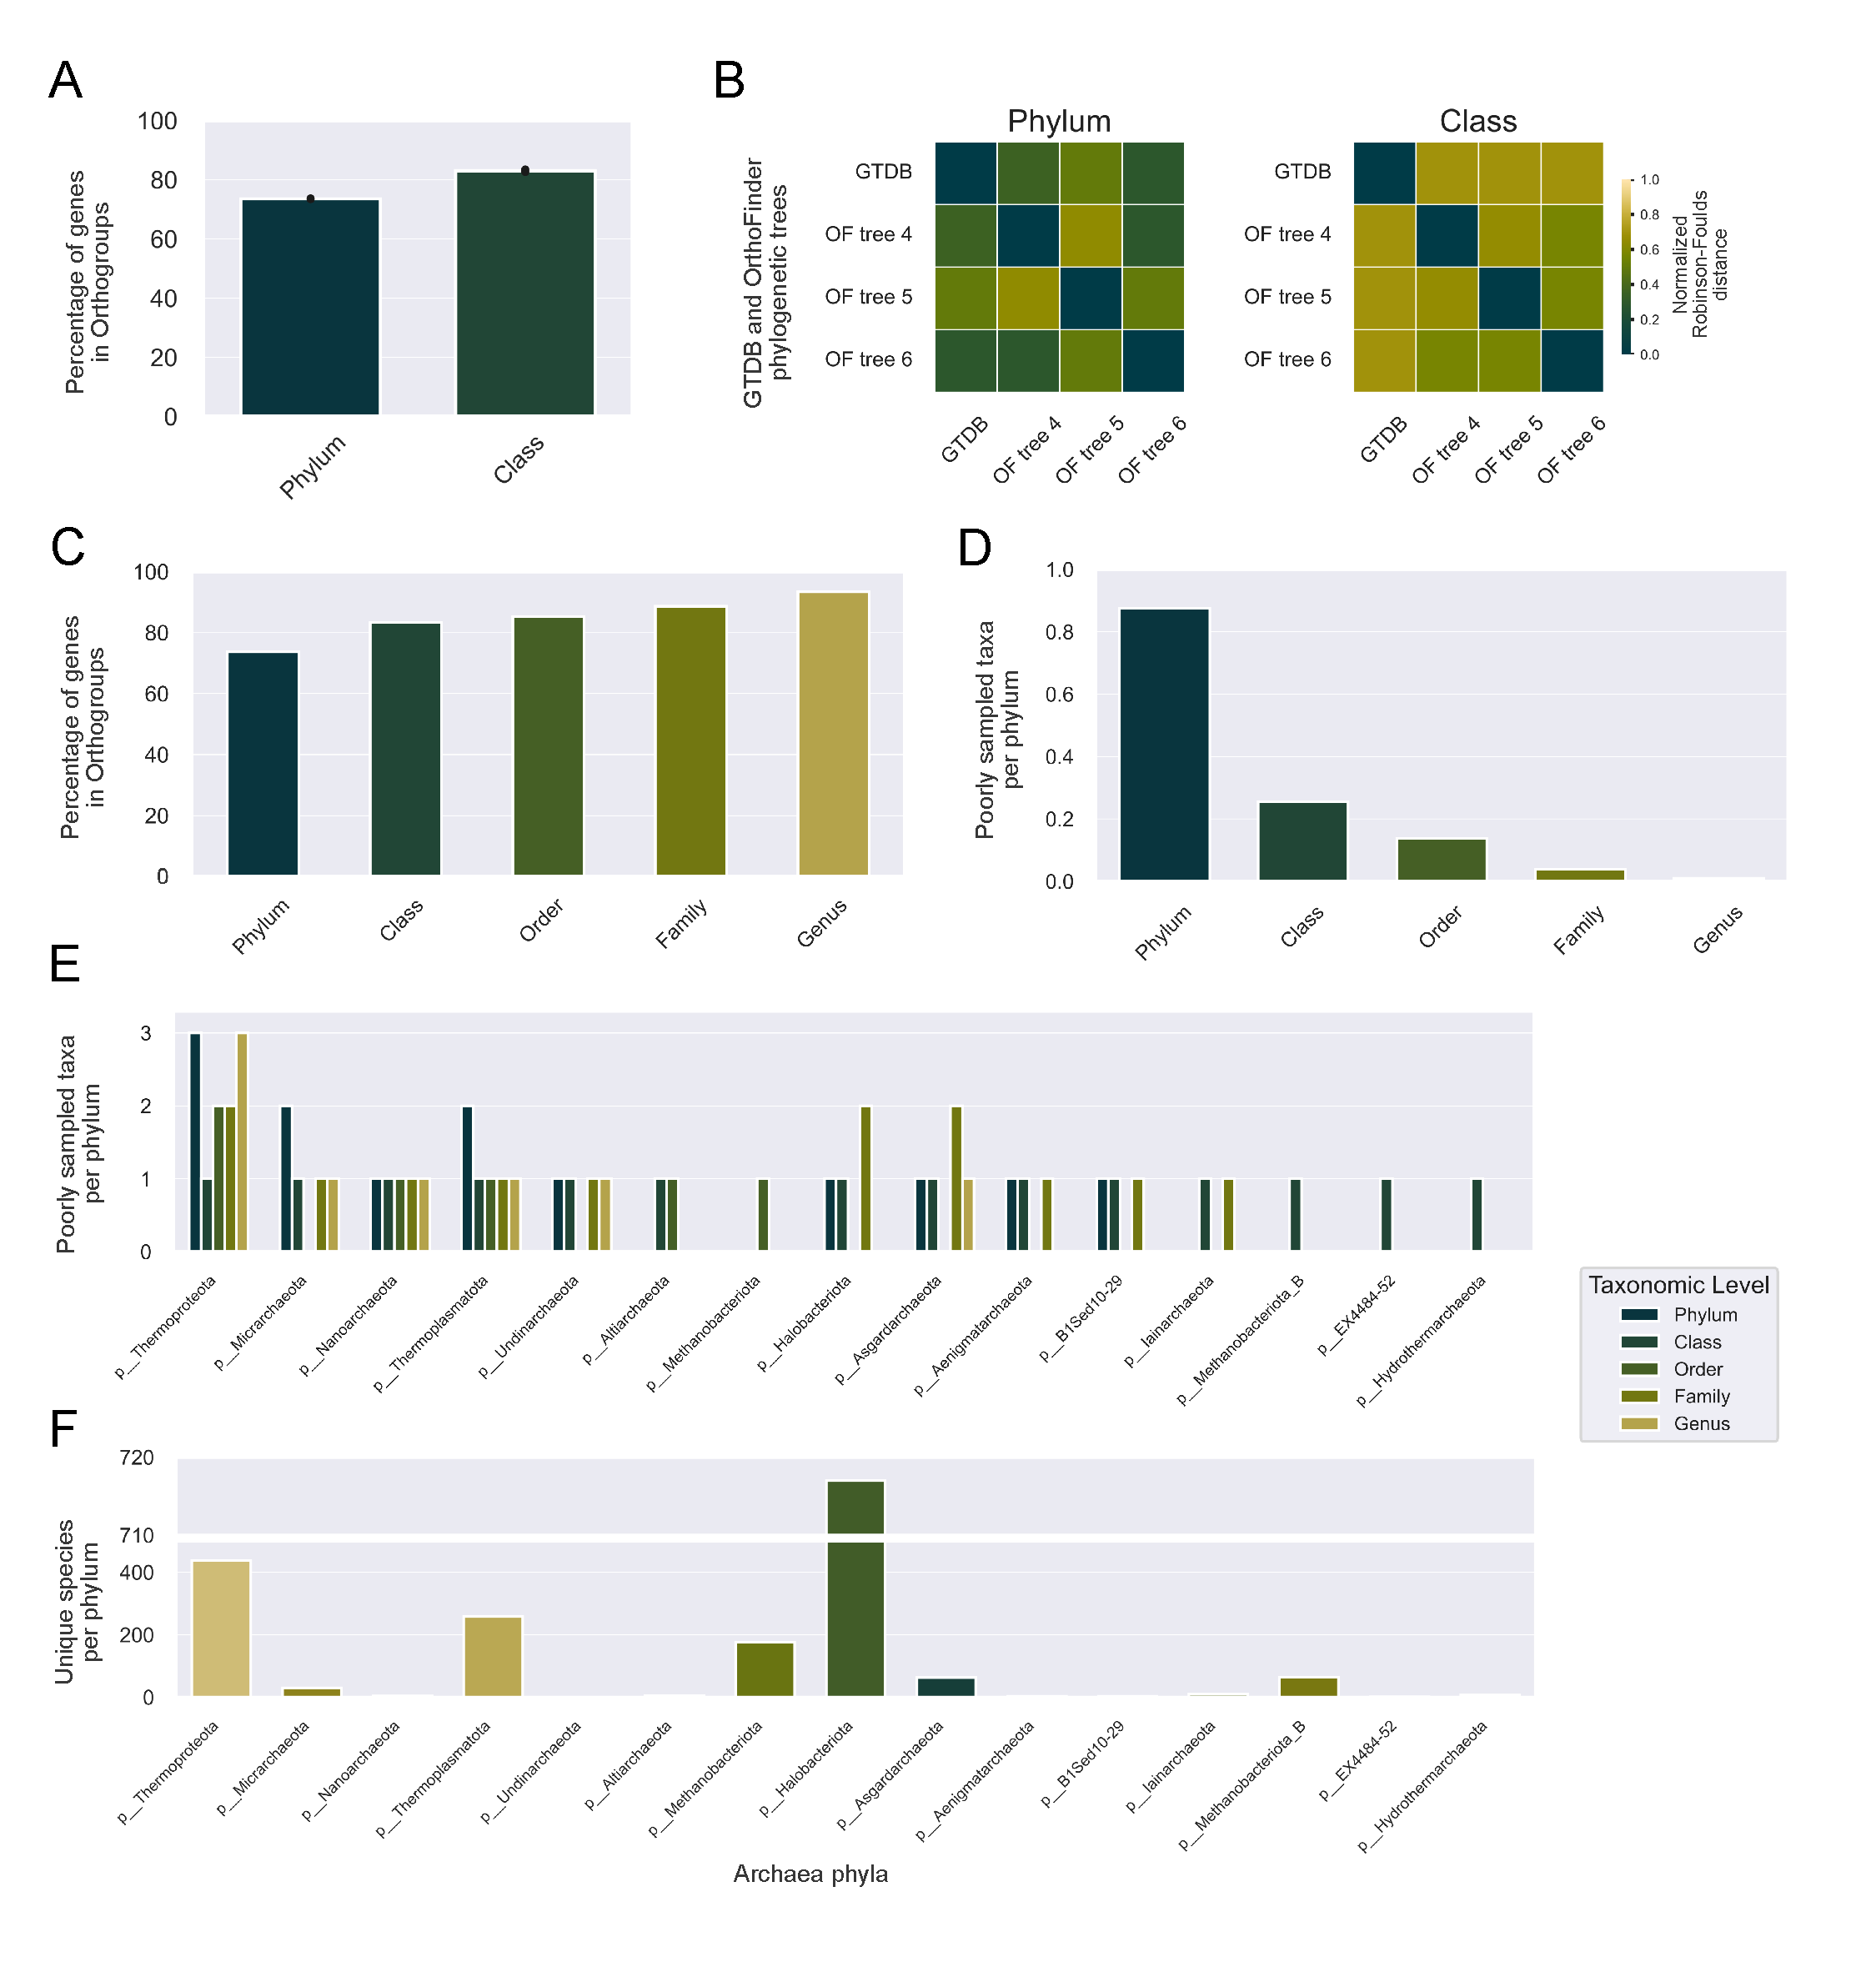
\includegraphics[width=0.97\textwidth]{fig2/fig2.pdf}
    \caption{Comparative genomics statistics of phylogenetic OrthoFinder (OF) analysis. (A) Shows the average percentage of genes assigned in orthogroups for the taxonomic levels of phylum and class for archaea. (B) Presents the Robinson-Foulds (RF) distance between the trees generated by OF as part of the aforementioned analyses, as well as their RF from the GTDB archaeal tree. (C) Compares the percentage of genes assigned in orthogroups for every archaeal taxonomic level. (D) Presents the normalized distribution of poorly sampled taxa for each taxonomic level analysis. (E) Detailed distribution of poorly sampled taxa for each taxonomic level analysis, per phylum, and (F) the number of unique species per phylum taxon.}
    \label{orthofinder_stats_figure}
\end{figure}   

A closer inspection of the statistics for individual taxa (Figure \ref{orthofinder_stats_figure}D and \ref{orthofinder_stats_figure}E) revealed that the percentage of poorly sampled genomes dropped below 5\% only at the family level (\ref{orthofinder_stats_figure}D). Interestingly, even though genomes belonging to particular phyla appear to be consistently categorized as "poorly sampled", this behavior cannot be linked to the number of species belonging to the same taxon. The Thermoproteota phylum, for example, has the highest count of "poorly sampled" species across all datasets, yet is the second richest archaeal phylum. Nanoarchaeota, on the other hand, whose genes are also consistently left out of orthogroups, comprise only of 4 species (Figure \ref{orthofinder_stats_figure}F). One has to take into account that species distribution remains uneven throughout the taxonomic levels, with some classes, orders, families, and genera that belong to the same phylum enriched more than others. Yet, with the decrease in genetic distance between species as datasets grow, and taxonomic levels become narrower, we would expect richer phyla to have a higher assignment of genes to OGs in narrower taxonomic levels.  

An initial comparison of the species trees produced by OF's STAG \cite{emms2018} and STRIDE \cite{emms2017} en-suite algorithms in Dendroscope \cite{huson2012} (found in Appendix Figures \ref{phylum_trees1} - \ref{gtdb_tree}) exposed unique tree topologies. Because of the significant missing gene orthology relationships at the phylum and class level, this did not come as a surprise. The more surprising finding came with calculating the Robinson-Foulds (RF) distance, a direct measure of phylogenetic tree similarity. RF calculates the number of nodes that are dissimilar between the phylogenetic trees under comparison, with lower values indicating a higher similarity degree. Even though the comparative genomics statistics results present the class level analyses as more-encompassing of orthology relationships, the inferred by OF species trees are more dissimilar than those for the phyla (Figure \ref{orthofinder_stats_figure}B). This could be rationalized by the fact that a smaller phylum dataset with longer genetic distances would be more likely to produce the same species tree topology. Nonetheless, it raises concerns about algorithms such as STRIDE using all genes, rather than only highly conserved ones, to infer a species tree. As Martinez-Gutierrez and Aylward \cite{martinez-gutierrez2021} have pointed out, \textit{"more genes and genomes do not necessarily improve phylogenetic accuracy"}. In light of this and considering our varying dataset sizes, we selected the GTDB domain-specific species trees for our downstream analysis.

\subsection*{Inferring ancestral genomes}
\addcontentsline{toc}{subsubsection}{Inferring ancestral genomes}

We wanted to utilize the full potential of the genomic data at hand for reconstructing ancestral metabolic networks, and avoid simplified approaches such as phylogenetic presence/absence profiles \cite{kreimer2008} or those using near-universal gene family distribution as filtering criteria \cite{xavier2021}. We therefore performed our phylogenetic analysis with OF \cite{emms2019, emms2015}, a comprehensive platform for comparative genomics that provides a standardized, accurate, fast, and scalable orthology inference approach. 

The relationship between number of each ancestor's descendants and ancestral genome size can be seen in Figure \ref{node_descendants_genomesize}. The number of descendants for node zero is a direct representation of the respective dataset size, as all descendants are utilized to infer its gene content. Leaf parents like nodes 3, 5, 10, 11, 12, 13, on the other hand, tend to have the smallest number of descendants. These relationships can be seen in the phylum-level tree topology of Figure \ref{node_descendants_genomesize} panel B. Of interest here is the uneven addition of new taxa to the various tree clades, with some clades experiencing rapid enrichment, while others remaining with few taxa. This unevenness could be a direct reflection of field sampling bias, but can be more likely be attributed to the culturability, and thus higher quality of genomic data, of specific taxa. For example, nodes 3 and 5, which represent a superphylum-level clade called DPANN, archaea with extremely small genome sizes and few cultured members \cite{dombrowski2019, dombrowski2020}, have very few descendants in all taxonomic-level datasets. What stands out the most, however, in Figure \ref{node_descendants_genomesize} panel, is the strong positive correlation between the inferred ancestral genome size and the number of descendants/initial sampling size, with a Pearson correlation coefficient close to 1 for all nodes. 

\begin{figure}[H]
    \centering
    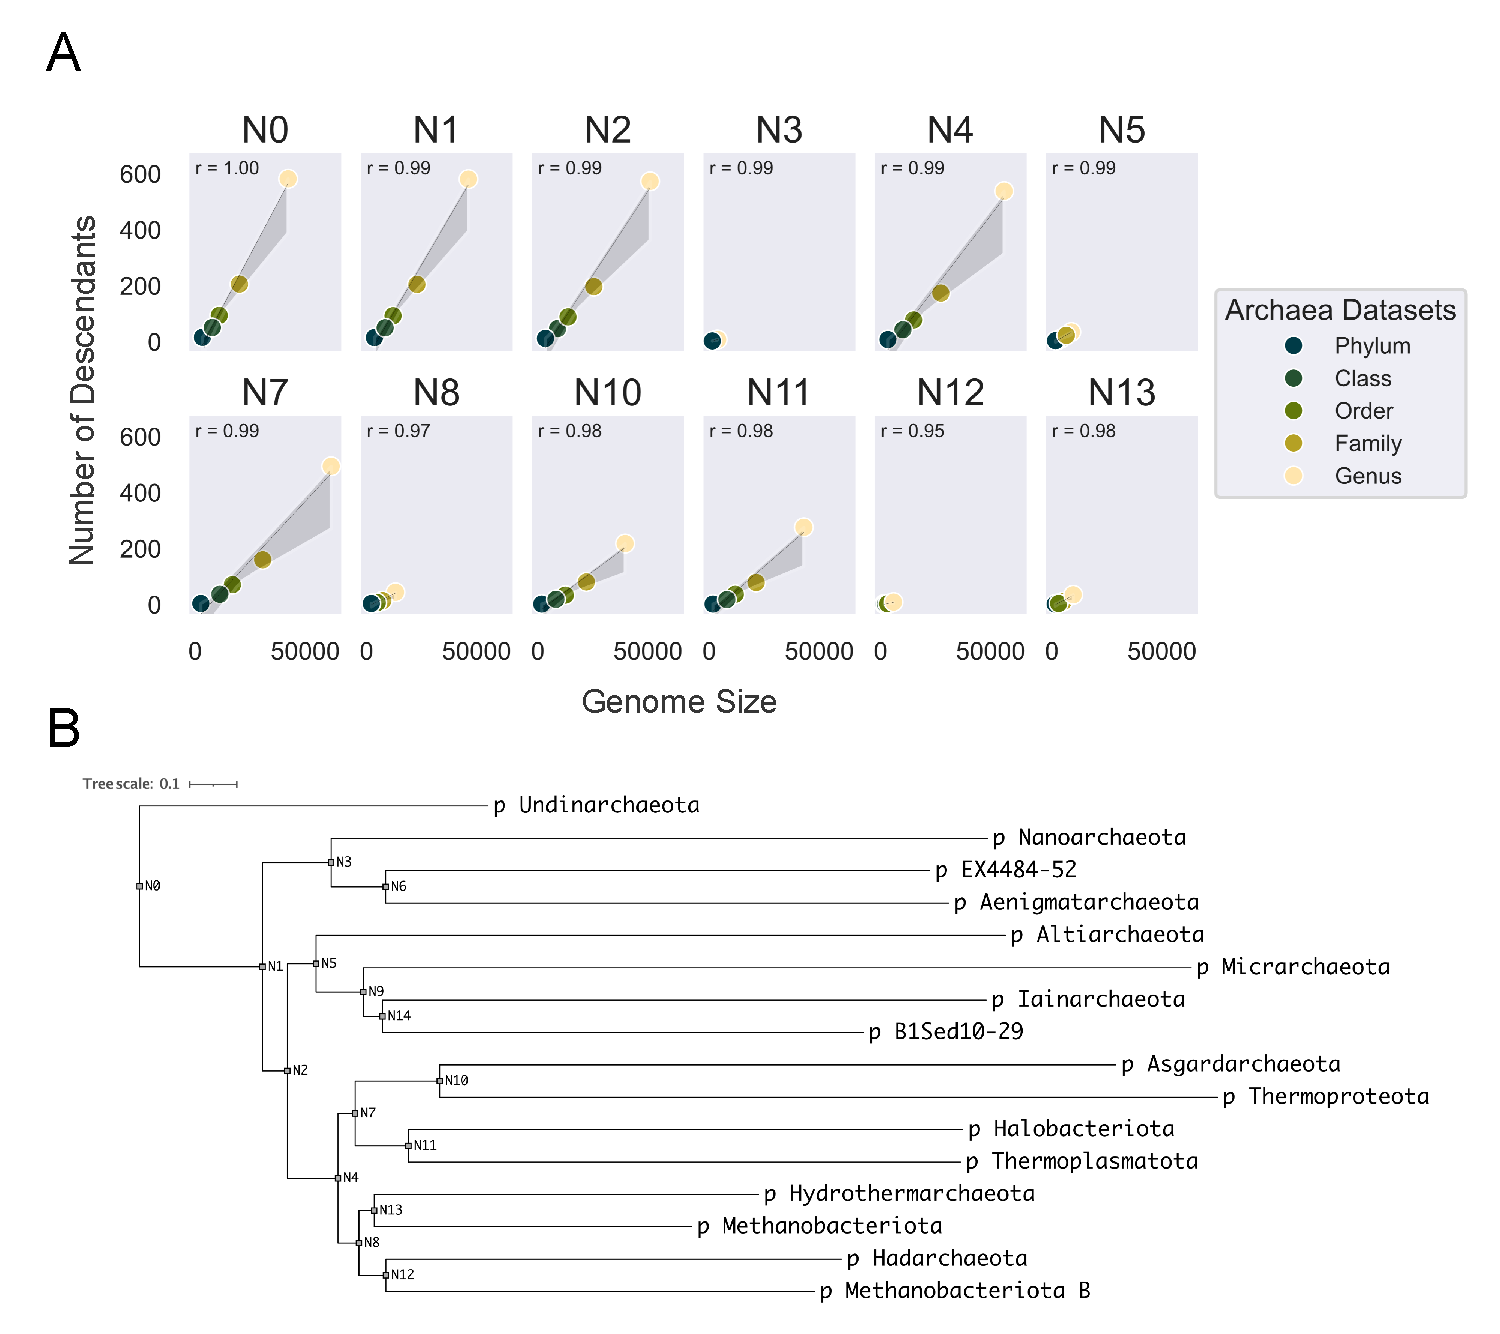
\includegraphics[width=0.95\textwidth]{fig1/fig1v2.pdf}
    \caption{Relationship between genome size and number of node descendants. (A) Shows the number of descendants of each node as a function of the inferred ancestral genome sizes, for all taxonomic levels of the archaea datasets. Colors are assigned to the five taxonomic levels, and turn lighter with narrower taxonomies. (B) Depicts the position of the nodes in the GTDB species tree, as well as their descendants. The phylum-level GTDB pruned tree has been used for simplification purposes. }
    \label{node_descendants_genomesize}
\end{figure}   


This relationship is not surprising, and can be attributed to the Duplication-Loss-Coalescence (DLC) parsimonious model for gene trees-species tree reconciliation OF utilizes. This model does not take into account horizontal gene transfer (HGT) events, and is known to overestimate gene content in ancestral genomes \cite{doolittle2003}. HGT, however, is not only omnipresent in prokaryotic evolution, but necessary for it \cite{ochman2000}. Especially when considering that any ancestral gene content reconstruction is necessarily incomplete, as the extinct gene families cannot be accounted for, it seems unreasonable that an ancient, last common ancestor would have the metabolic versatility of the entire modern biosphere. The inferred ancestral genomes of this study should therefore be considered with caution at this stage. Another model, the Duplication-Transfer-Loss (DTL) model, which accounts for HGT, is able to mitigate the tendency to infer unrealistically large ancestral genomes, getting bigger with each added genome, in the absence of HGT \cite{doolittle2003}. We therefore plan to redo our analysis by employing the DTL model, which has been shown to be more realistic and robust to gene tree uncertainty \cite{szollosi2013, szollosi2015}.

\subsection*{Ancestral Genome Functional Annotation}
\addcontentsline{toc}{subsubsection}{Ancestral Genome Functional Annotation}

For the metabolic network reconstruction of the ancestral genomes, we functionally annotated a single sequence for each of the OGs inferred to be present in the respective ancestor node. We based this decision on the rationale that an OG comprises genes that have descended from a single gene in the last common ancestor (LCA) of a group of species, and that sequences within the same OG are evolutionarily closer to each other than to sequences outside of that OG. Yet, the OGs OrthoFinder infers include both orthologs and paralogs, and functional annotation is known to be most reliable when based on orthologs, as they are expected to retain function more often than paralogs \cite{gabaldon2013a}. To assess the impact of choosing an OG representative sequence on functional annotation, we compared the functional annotations of the first sequence within each OG against the medoid sequence of the same OG (Figure \ref{waffleplot}). The medoid sequence is the sequence with the shortest genetic distance to all other sequences in the OG, and is therefore considered a better representative of the OG than the first---essentially a random---sequence. Since OF solves the gene length bias in orthogroup inference---which tends to cluster sequences of similar length together---the produced OGs include sequences of varying lengths. It may therefore be beneficial to perform a multiple sequence alignment for each OG, in the future, before choosing a representative sequence for functional annotation. Even though we do not check here for the length of the representative sequence relative to the median sequence length of an OG, there may be a selection bias towards lengths that are more common in the OG, which is also not necessarily erroneous. 

Figure \ref{waffleplot} presents the comparison statistics from the functional annotation of the two sequences belonging to the same OG in the form of a waffle plot; the dataset used for this part of the study is the phylum level archaeal one run against the Archaea (2157) eggNOG v5 database. EggNOG-mapper takes the protein sequences we provide and performs functional annotation after sequence alignment, based on the best hit. Out of 2849 OGs, for 68\% the first and medoid sequences differed, for 26\% they were the same, and 6\% were individual hits (Fig. \ref{waffleplot} orange), meaning that eggNOG-mapper found a match in the database for only one of them. Henceforth, we compare KEGG reaction and EC assignment only for different hits. Most hits do not correspond to neither a reaction ID nor EC number (Fig. \ref{waffleplot} gray blocks). Considering that the GTDB data used in our study only contain sequences predicted by Prodigal to be protein-coding, the absence of a match for the majority of the sequences is perplexing; it raises questions regarding the incompatibility between tools and databases used throughout the globe for genomic and metagenomic workflows. For hits that do find a match, 73\% share the same KEGG reaction ID, and another 71\% share the same EC number (Fig. \ref{waffleplot} purple and blue). With regard to the KEGG EC assignment, if we relax our constraints and compare EC assignments up to the third digit, which specifies the nature of the reaction \cite{mcdonald2009}, the percentage of shared EC assignments increases to 79\%. This simple statistical analysis stresses how important the choice of representative sequence is for functional annotation, even for related sequences that may have descended from the same gene. 

\begin{figure}[H]
    \centering
    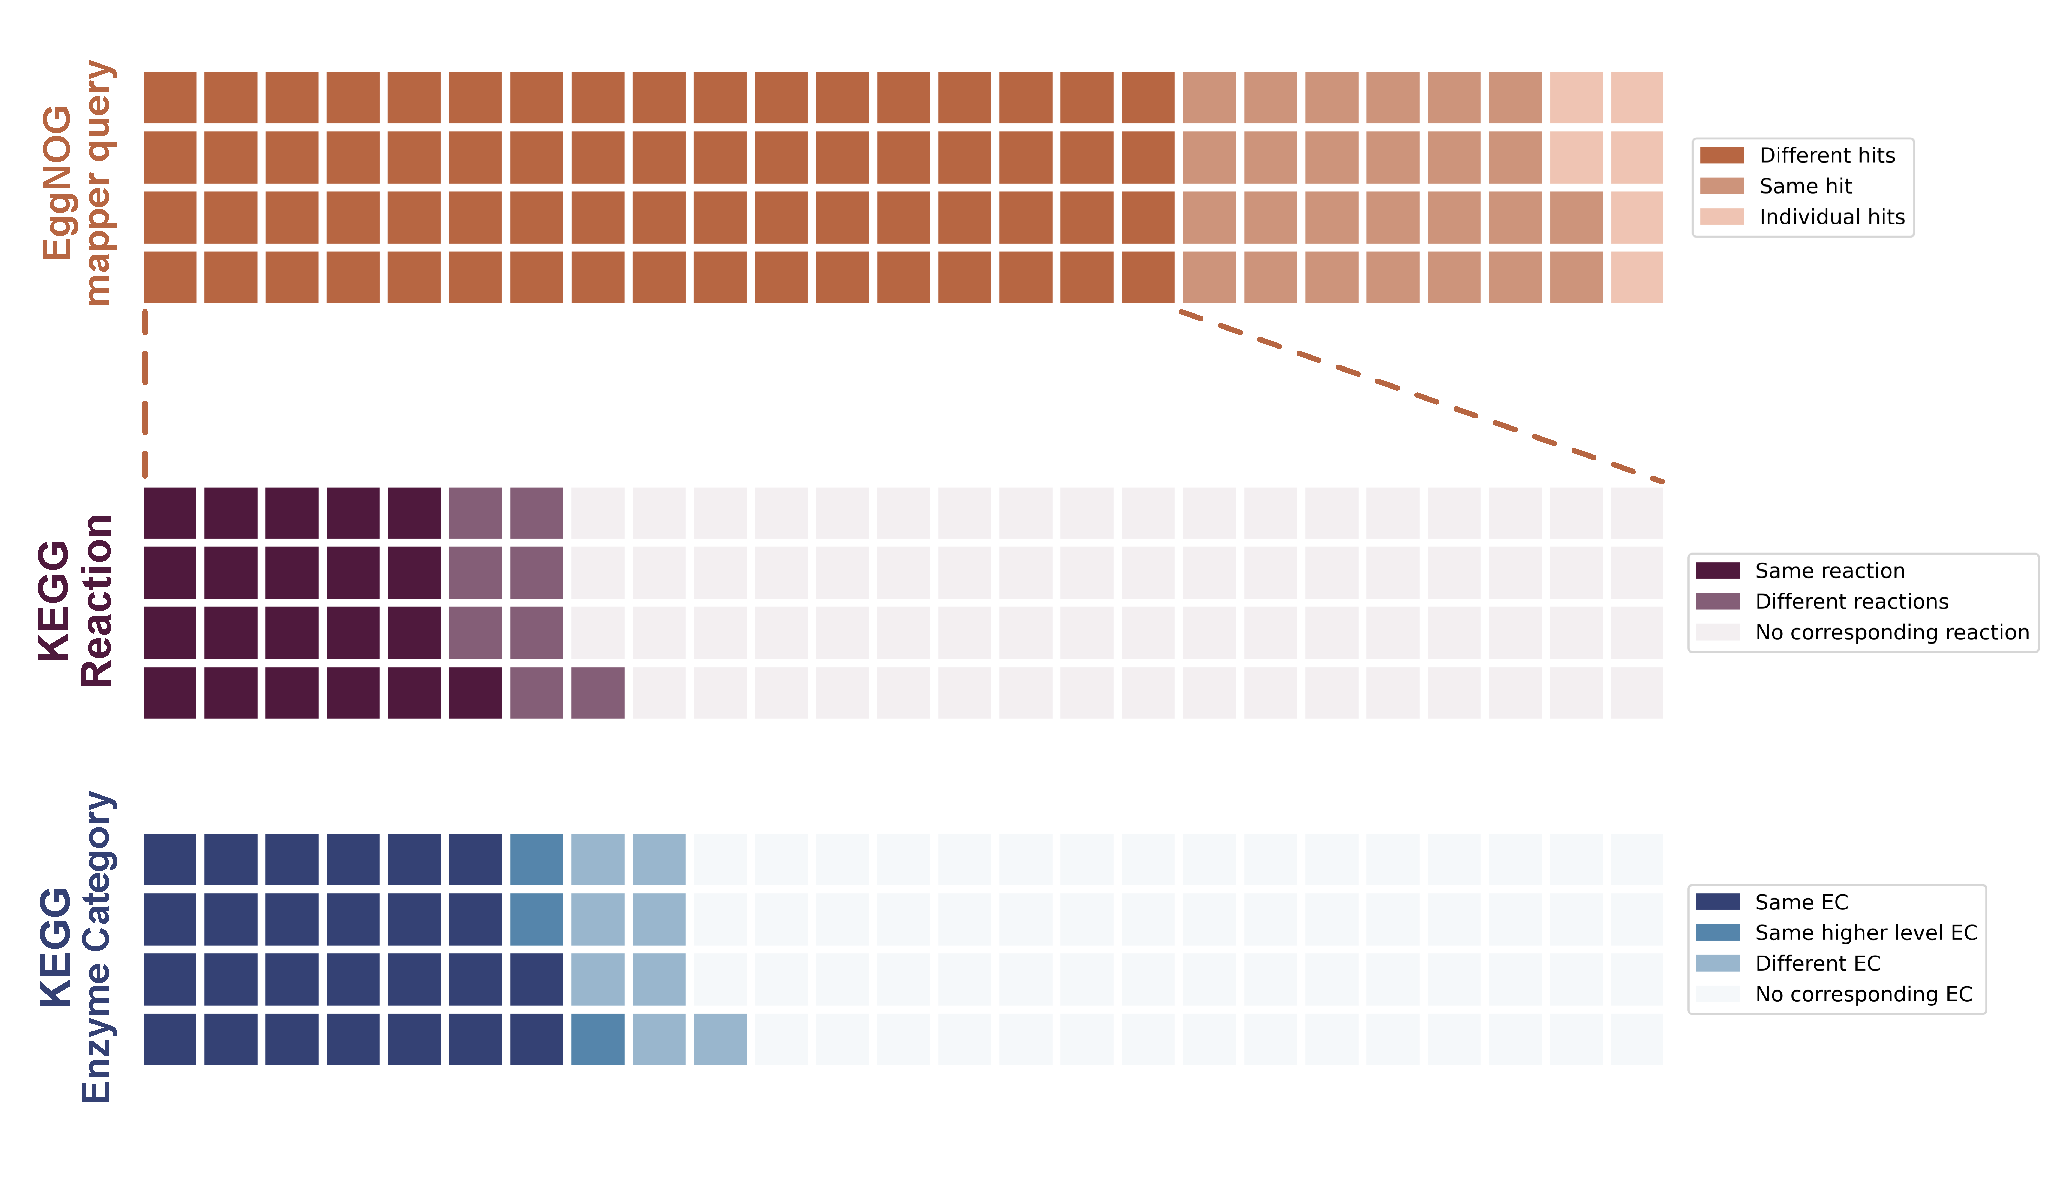
\includegraphics[width=0.95\textwidth]{waffleplot.pdf}
    \caption{Comparison of functional annotations between the first and medoid sequence of each ancestral Node zero (N0) for the archaea phylum level dataset. The waffle plot shows the percentage of a quantity---orange for number of OGs (used as a proxy for number of hits), purple for KEGG reaction number of different queries, and blue for KEGG enzyme commission (EC) number of different queries.  
     Every axis---orange, purple, and blue---shows a different statistic}
    \label{waffleplot}
\end{figure}   

For our inferred ancestral genomes belonging to the archaea phylum and class level datasets, the medoid sequence was calculated and utilized for OG functional annotation. For the rest of the datasets (found in Table \ref{datasets}), we sampled a hundred sequences from each OG at random, and calculated the medoid only for those. Since the medoid is calculated by pairwise alignment of all sequences in an OG, the computational burden increases according to the Gauss's summation formula (Equation \ref{eq:alignments}), where \textit{n} is the number of sequences. As our datasets grow in size, the number of sequences attributed to each OG increases to a point where calculating the medoid becomes extremely time-consuming. For example, an OG with 1000 sequences---which becomes common in our larger datasets---would require 500,500 pairwise alignments. We therefore opted for a computationally tractable approach, calculating the medoid for a hundred randomly sampled sequences for OGs larger than that. Instead of calculating the medoid for all OGs, we could also have annotated all sequences of an OG, and then choose the most common eggNOG OG (eggNOG orthogroup) or COG (cluster of orthologous genes) category as the representative one for the OG, as done by Xavier et al. \cite{xavier2021}. 

\begin{equation}
    \label{eq:alignments}
    \sum_{i=1}^{n} i = \frac{n(n+1)}{2}
\end{equation}

As mentioned above, the functional annotation does not only depend on the sequence itself, but on the database against which it is aligned. A feature of eggNOG-mapper version 2 \cite{cantalapiedra2021} allows for the generation of taxon-specific eggNOG databases. We therefore generated three databases spanning the prokaryotic domain, one for the Archaea (2157), one for Bacteria (2), and a general one including both domains (2157, 2). We then performed functional annotation of genes predicted to be present for certain internal tree nodes (presented in Figure \ref{node_descendants_genomesize}) against the domain-specific and the general eggNOG databases, chose for the best hit between the two runs, as described in the Methods section, and reconstructed each metabolic network based on the KEGG reaction IDs assigned by eggNOG-mapper for each best hit. Extant genomes were annotated only against the general eggNOG database. 

We also tried performing functional annotation of entire OGs, instead of single protein sequences, with profile hidden markov models (HMMs), as a more sensitive, probabilistic approach. In contrast to traditional substitution matrices, such as the BLOSUM matrix \cite{henikoff1992} we utilized to determine the medoid, profiles are position-specific scoring models and take into account specific---to each sequence---conservation patterns \cite{mount2009, gribskov1987}, and can therefore offer enhanced alignment and functional annotation quality. However, this methodology is even more time-consuming than simply calculating the medoid, and was not feasible with our current computational resources. In future analyses, we plan to use HMMs for functional annotation of the OGs, and compare the results with those obtained by the medoid method.

\subsection*{Metabolic Network Reconstruction}
\addcontentsline{toc}{subsubsection}{Metabolic Network Reconstruction}


One of the first things we noticed when mapping our inferred reaction IDs to the KEGG database was the absence of multiple IDs per dataset and often incomplete or missing fields, leading to inconsistent information between reactions; for example, some reactions include the KEGG module or pathway, while others do not. Even though the KEGG databases provide a valuable resource for the field of bioinformatics and metabolism modeling \cite{kanehisa2000}, it was primarily designed for visualization purposes, and its reactions are often unbalanced \cite{wrzodek2013} and can be even elementally inconsistent \cite{goldford2024}. For these reasons, we utilized the database compiled by Goldford et al. (2024) \cite{goldford2024}, which extends the KEGG reactions database by excluding elementally inconsistent reactions and adding detailed organic and inorganic cofactor dependencies from various other databases. 

To inspect the connectivity of the reconstructed metabolisms of putative, ancient microorganisms, we visualized the networks using iPath \cite{darzi2018}, an interactive metabolic pathway explorer that is based on four KEGG global maps. The hypothetical metabolic potential of LACA for the family-level archaea dataset can be seen in Figure \ref{fam4arc_metnet}, while the rest of LACA-inferred metabolic networks can be found in Appendix Figs. \ref{phy4arc_metnet} - \ref{gen4arc_metnet}. Even at the phylum-level, the network seems relatively well-connected, with isolated reactions being dispersed across the entire map. The smallest of the reconstructed metabolic networks, after all, contains 1192 reactions. 

\begin{figure}[H]
    \centering
    \includegraphics[width=0.98\textwidth]{metabolism/fam_arc_N0.pdf}
    \caption{Reconstruction of LACA's metabolic network from extant life, for the family-level archaea dataset. In black: enzymes and metabolic pathways that were inferred to be present in LACA.}    
    \label{fam4arc_metnet}
\end{figure}

%Another drawback of using KEGG Orthology (KOs), instead of COGs---which correspond to wider gene families---\cite{tatusov2003}, to construct hypothetical metabolism models of ancient microorganisms, is that gene families that were likely present in those organisms are divided into multiple KO families that appear in particular taxonomic groups and may only be inferred for younger ancestors \cite{moody2024}.

Phylogenetic-based metabolic network reconstruction enables the mapping of genetic information to genome distance from the tree root. We aimed to explore the emergence and evolution of individual ECs across the tree of life, a topic that has not been previously investigated. For this, we acquired the distance of all nodes from the tree root and used it as a proxy for evolution. All enzyme categories are present in the reconstructed LACA metabolism (Figure \ref{ec_vs_rootdist_fam}B). The relative abundance of ligases and oxidoreductases is higher in the inferred ancient metabolisms, while that of transferases declines. Lyases and isomerases are universally more limited and do not become enriched over time. This divergence may indicate a different rate of innovation for various ECs or suggest that specific types of enzymes are more prone to either loss or gain.

No other significant differences or patterns are observable, so it may be beneficial to divide the tree into multiple clades and track EC evolution within specific groups of species rather than across the entire tree. This approach will be especially important if we increase the deep branch resolution by reconstructing the metabolic networks of all possible internal tree nodes. Even though the relative abundance of the six EC categories varies between inferred and extant microorganisms, their distribution across the tree follows a similar pattern, reflecting the species distribution across the tree (Fig. \ref{ec_vs_rootdist_fam}A). Small variations, such as the increase in transferases at a distance of around 1.5 from the tree root, may indicate an enrichment of this enzyme category in certain species, possibly due to specialization or an evolutionary advantage.

\begin{figure}[H]
    \centering
    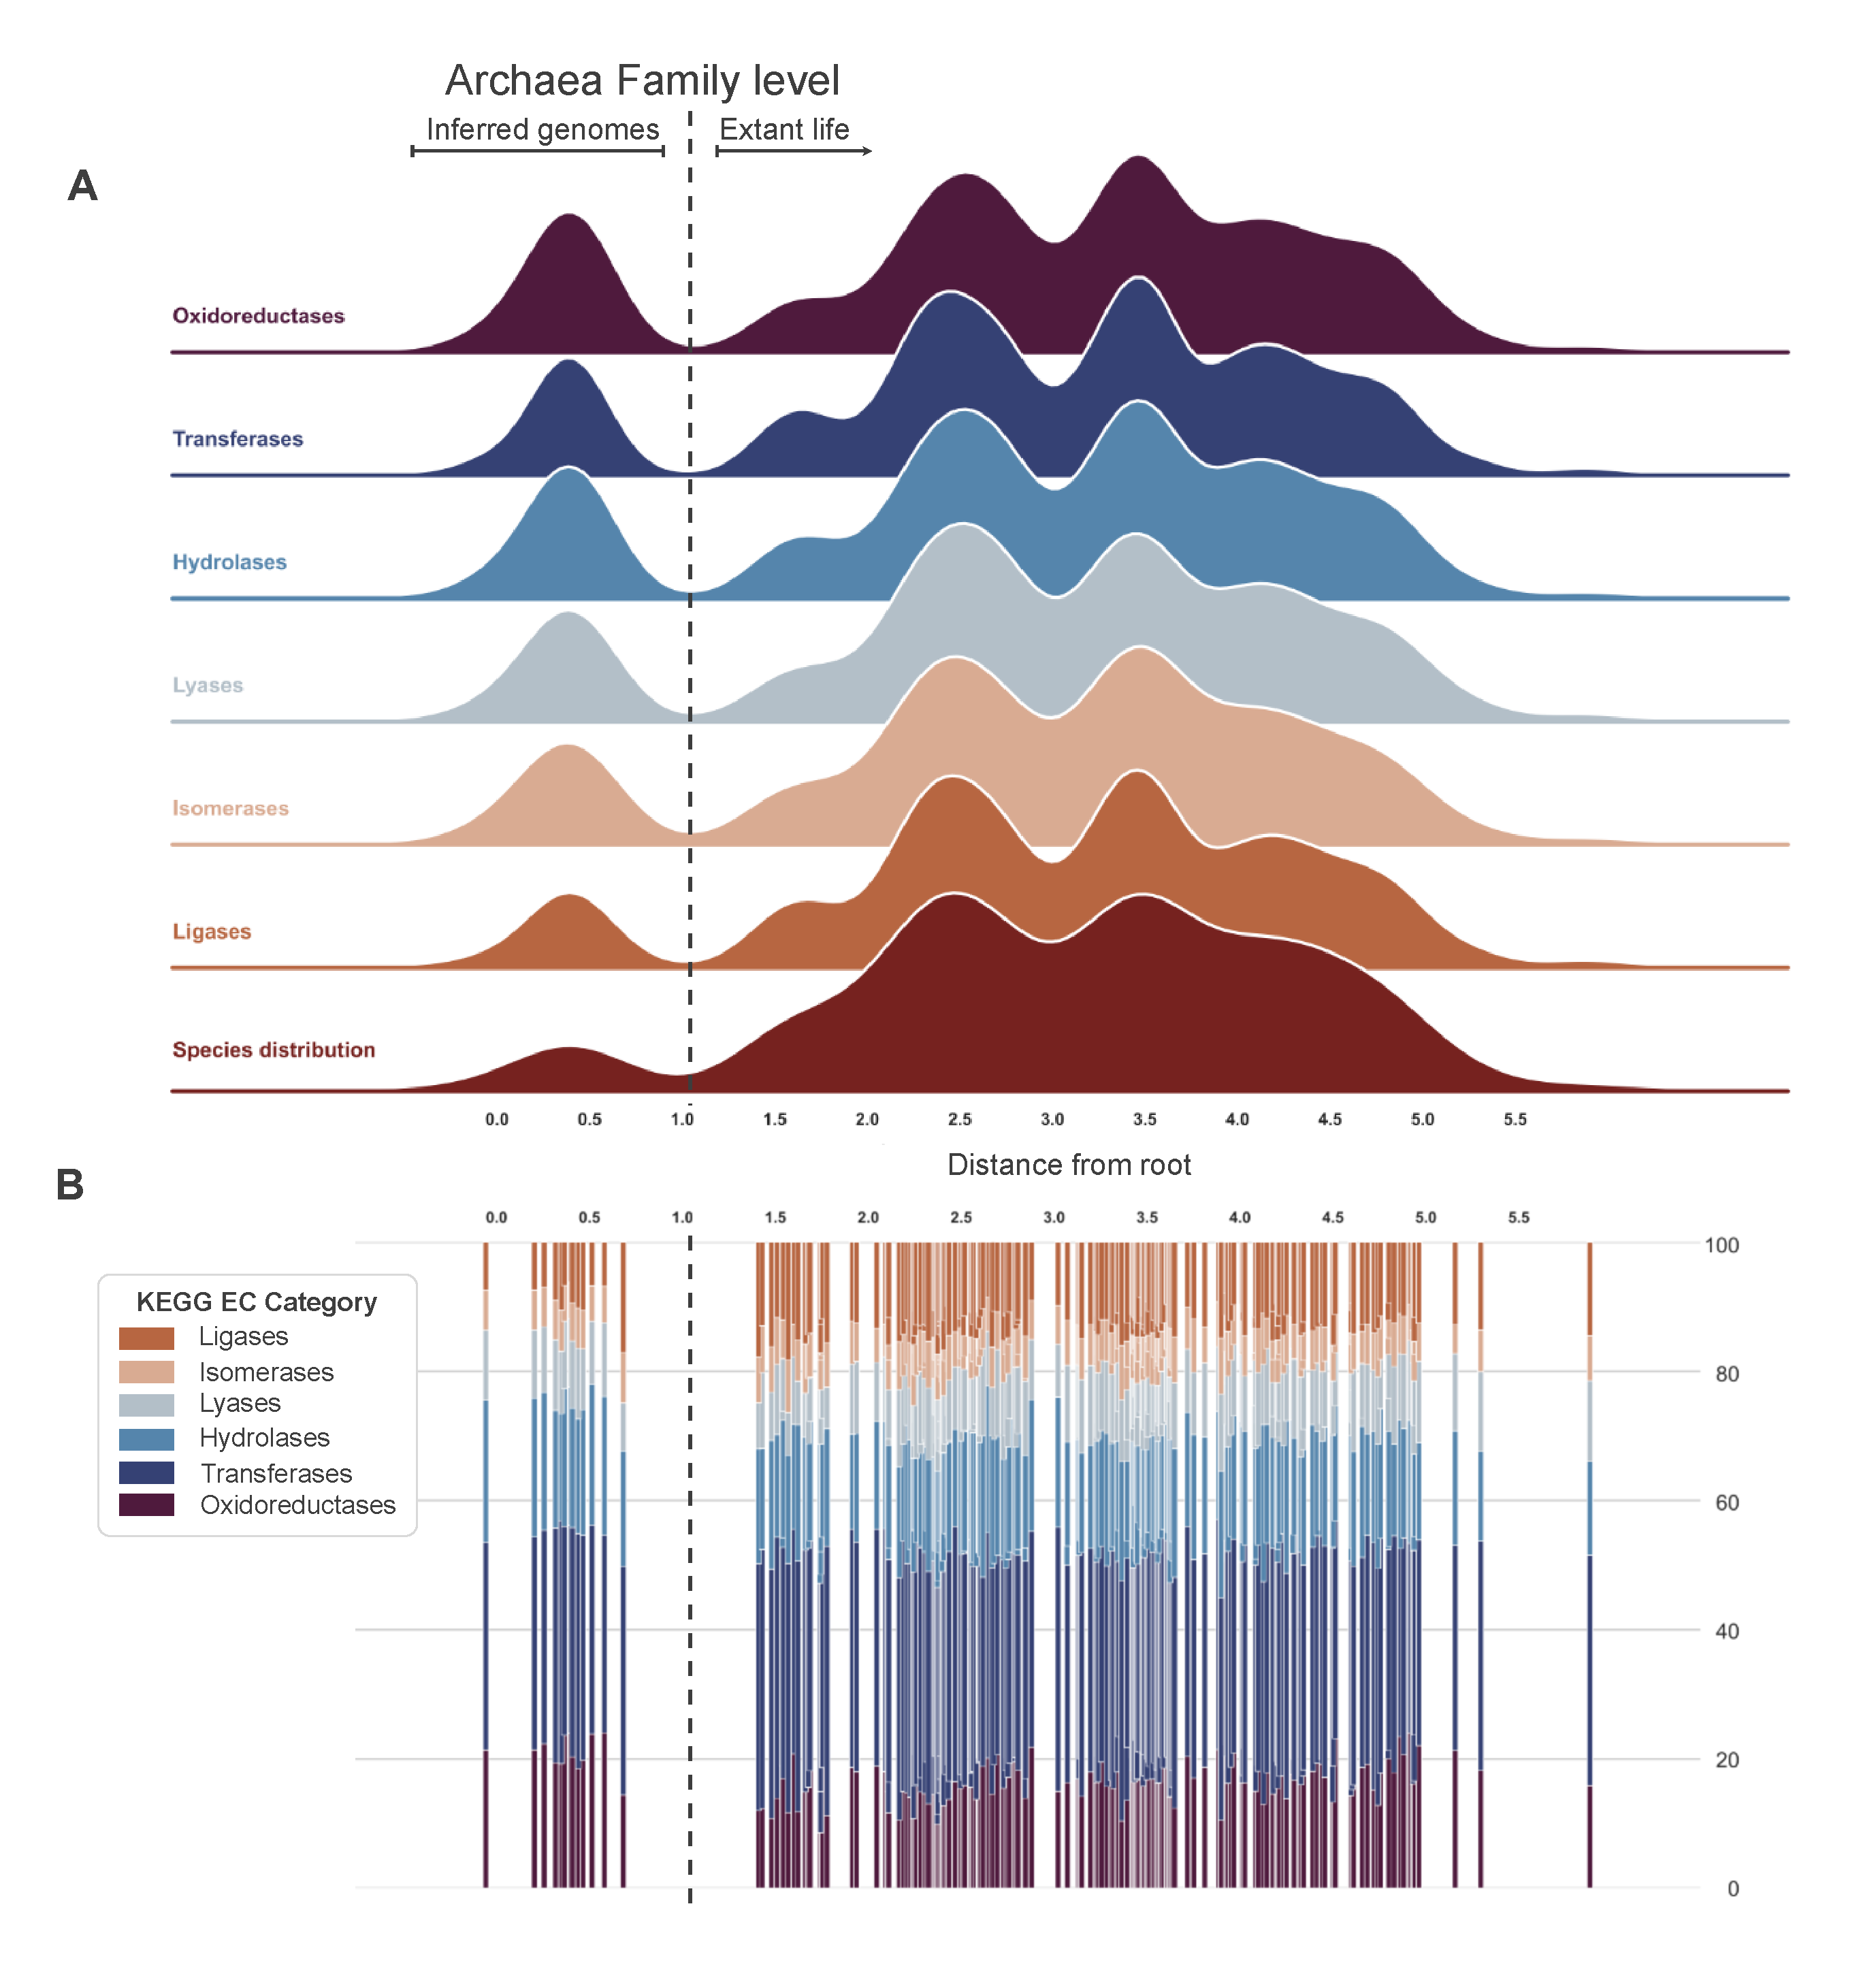
\includegraphics[width=0.9\textwidth]{ridgeplots/ec_vs_rootdist_fam.pdf}
    \caption{Evolution of individual enzyme categories for the family-level archaea dataset. The dashed line separates the inferred ancient metabolisms, on the left, from the extant ones, on the right. The ridgeplot of panel (A) displays the distribution of each category as a function of distance from the tree root, with the last axis presenting the species distribution. (B) shows the relative abundance of each category at that particular distance as a stacked barplot.}
    \label{ec_vs_rootdist_fam}
\end{figure}  

\subsection*{Metabolic Network Expansion}
\addcontentsline{toc}{subsubsection}{Metabolic Network Expansion}

** gray covers the reactions of the expanded network. They always will be less populated than the black ones. The blue dots (scope) include the red dots (seed set).

\begin{figure}[H]
    \centering
    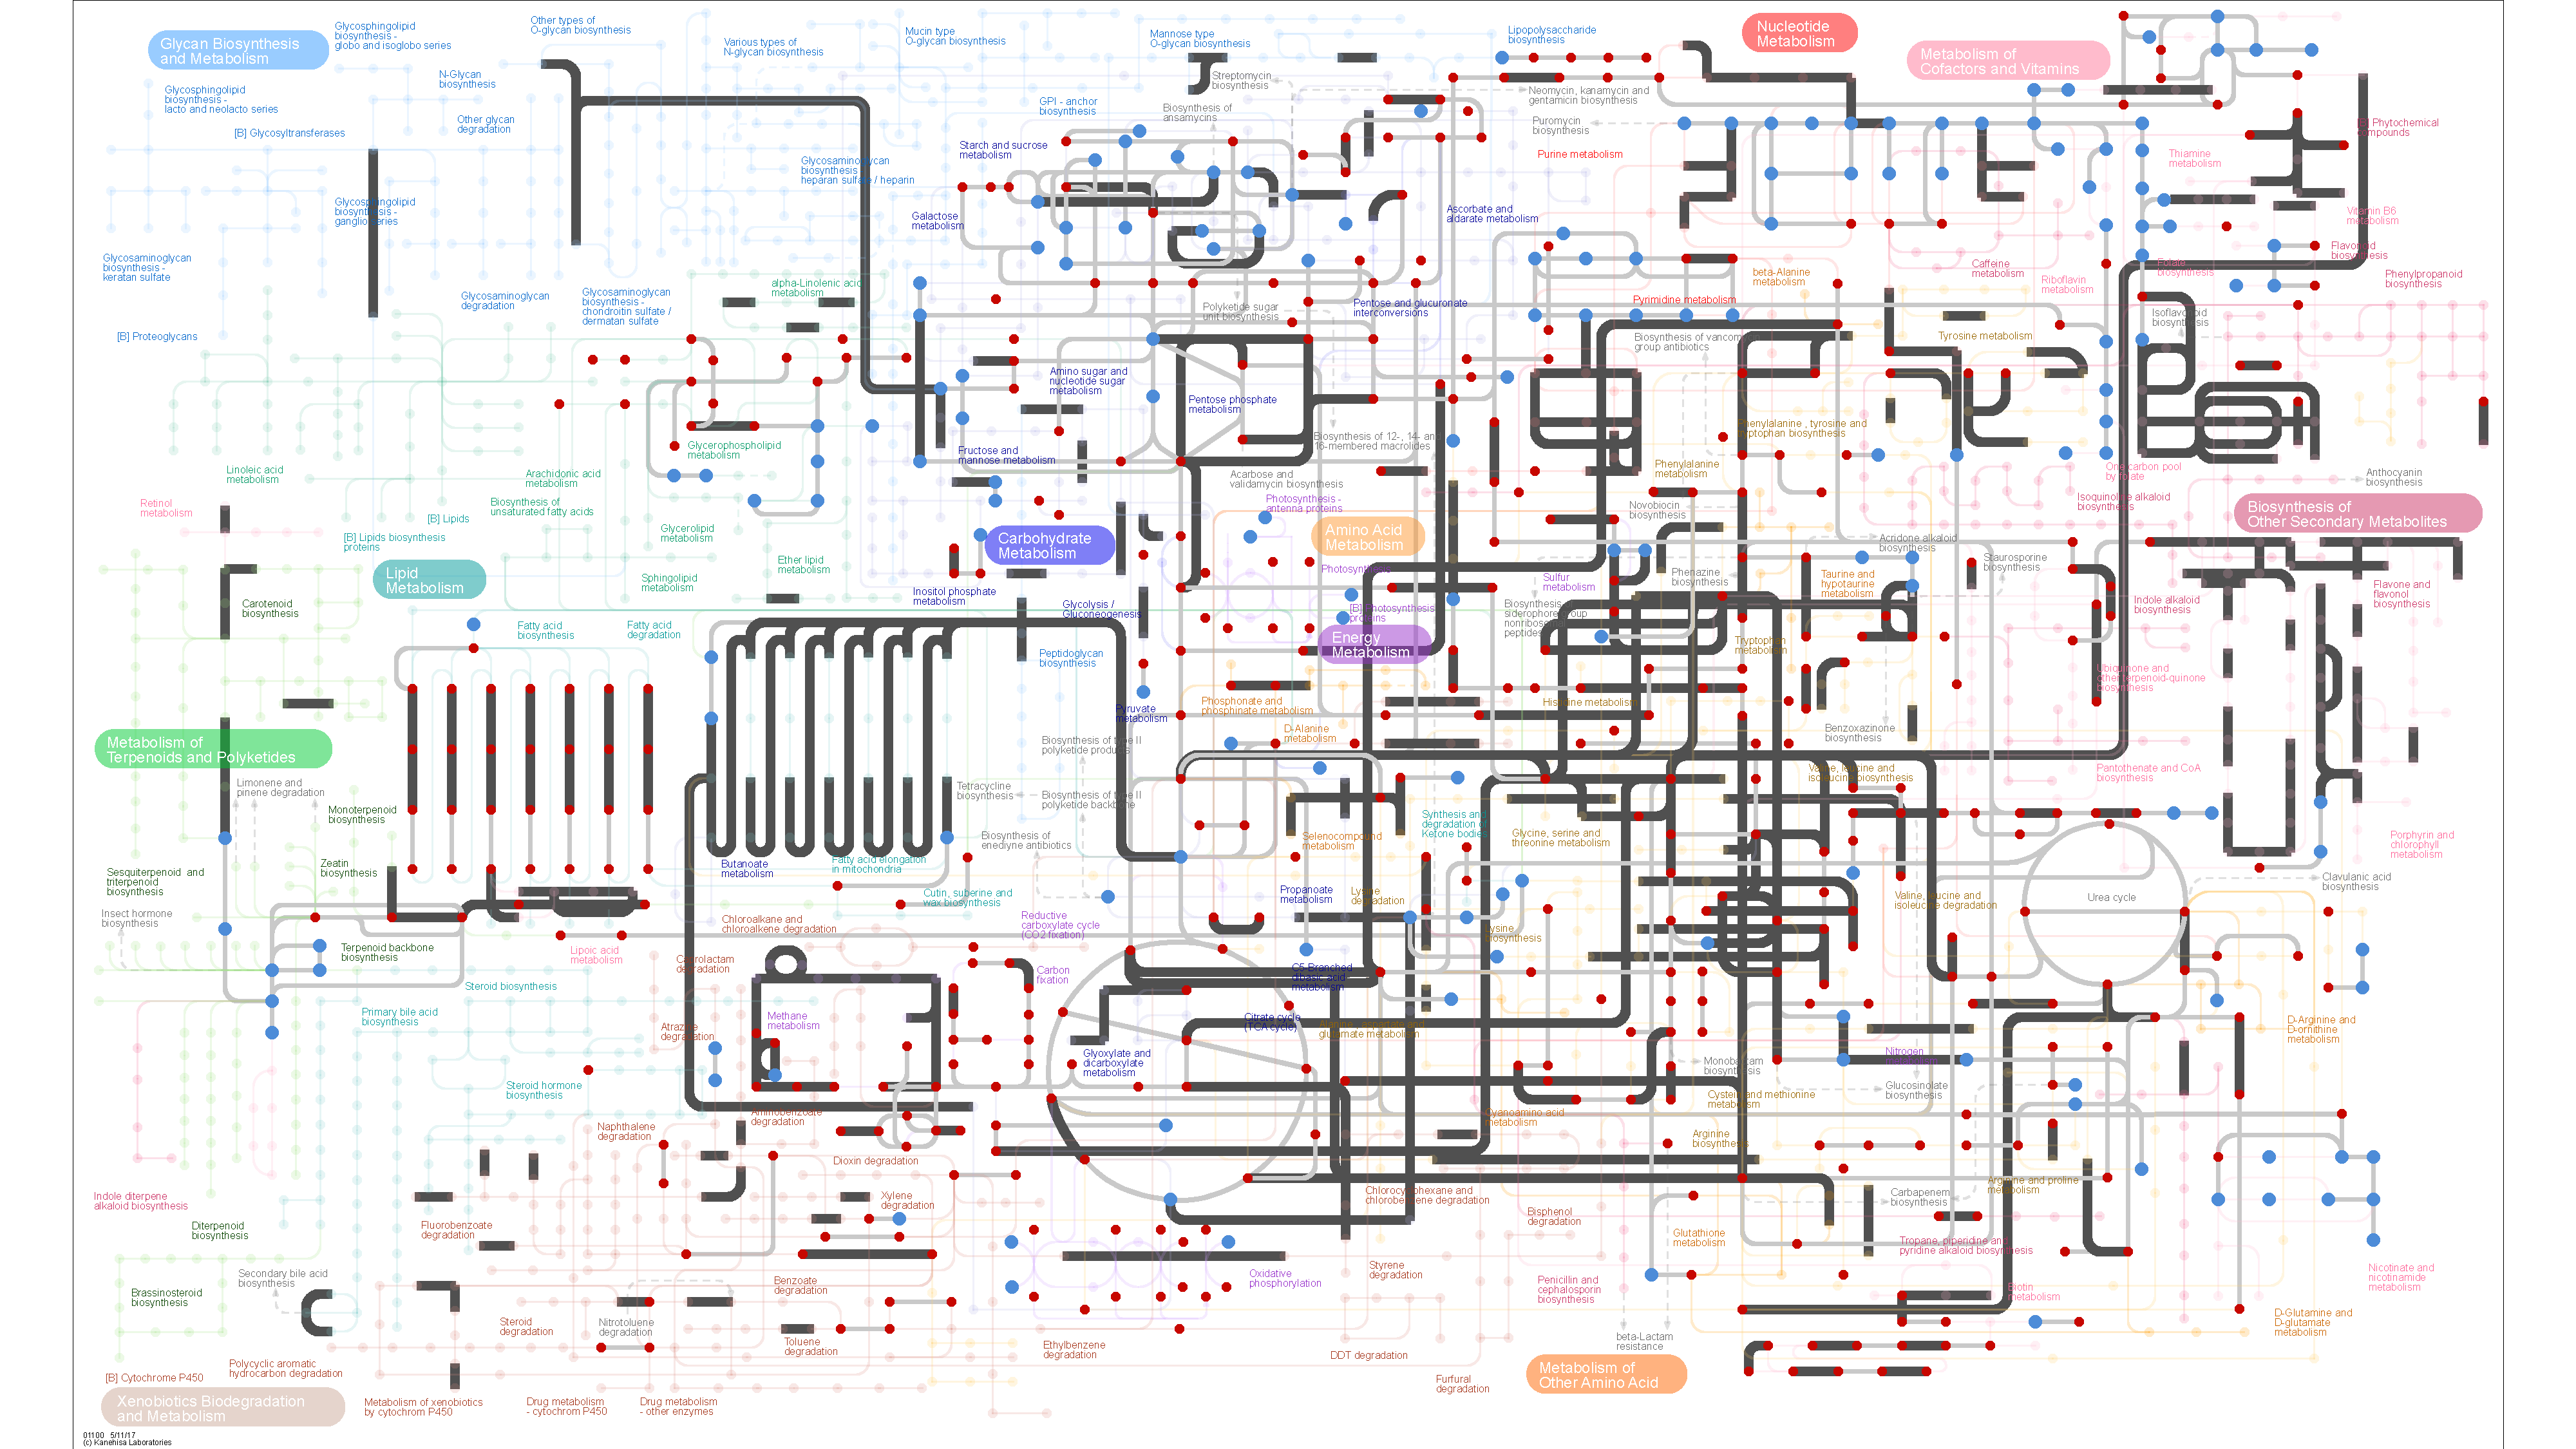
\includegraphics[width=0.98\textwidth]{metabolism/fam_N0_exp.pdf}
    \caption{Reconstruction of LACA's metabolic network from extant life, for the family-level archaea dataset. In black: enzymes and metabolic pathways that were inferred to be present in LACA. In gray: enzymes and metabolic pathways of the expanded network. Red dots: seed set compounds present in the reconstructed network. Blue dots: scope compounds after network expansion.}    
    \label{fam4arc_metnetexp}
\end{figure}

\begin{figure}[H]
    \centering
    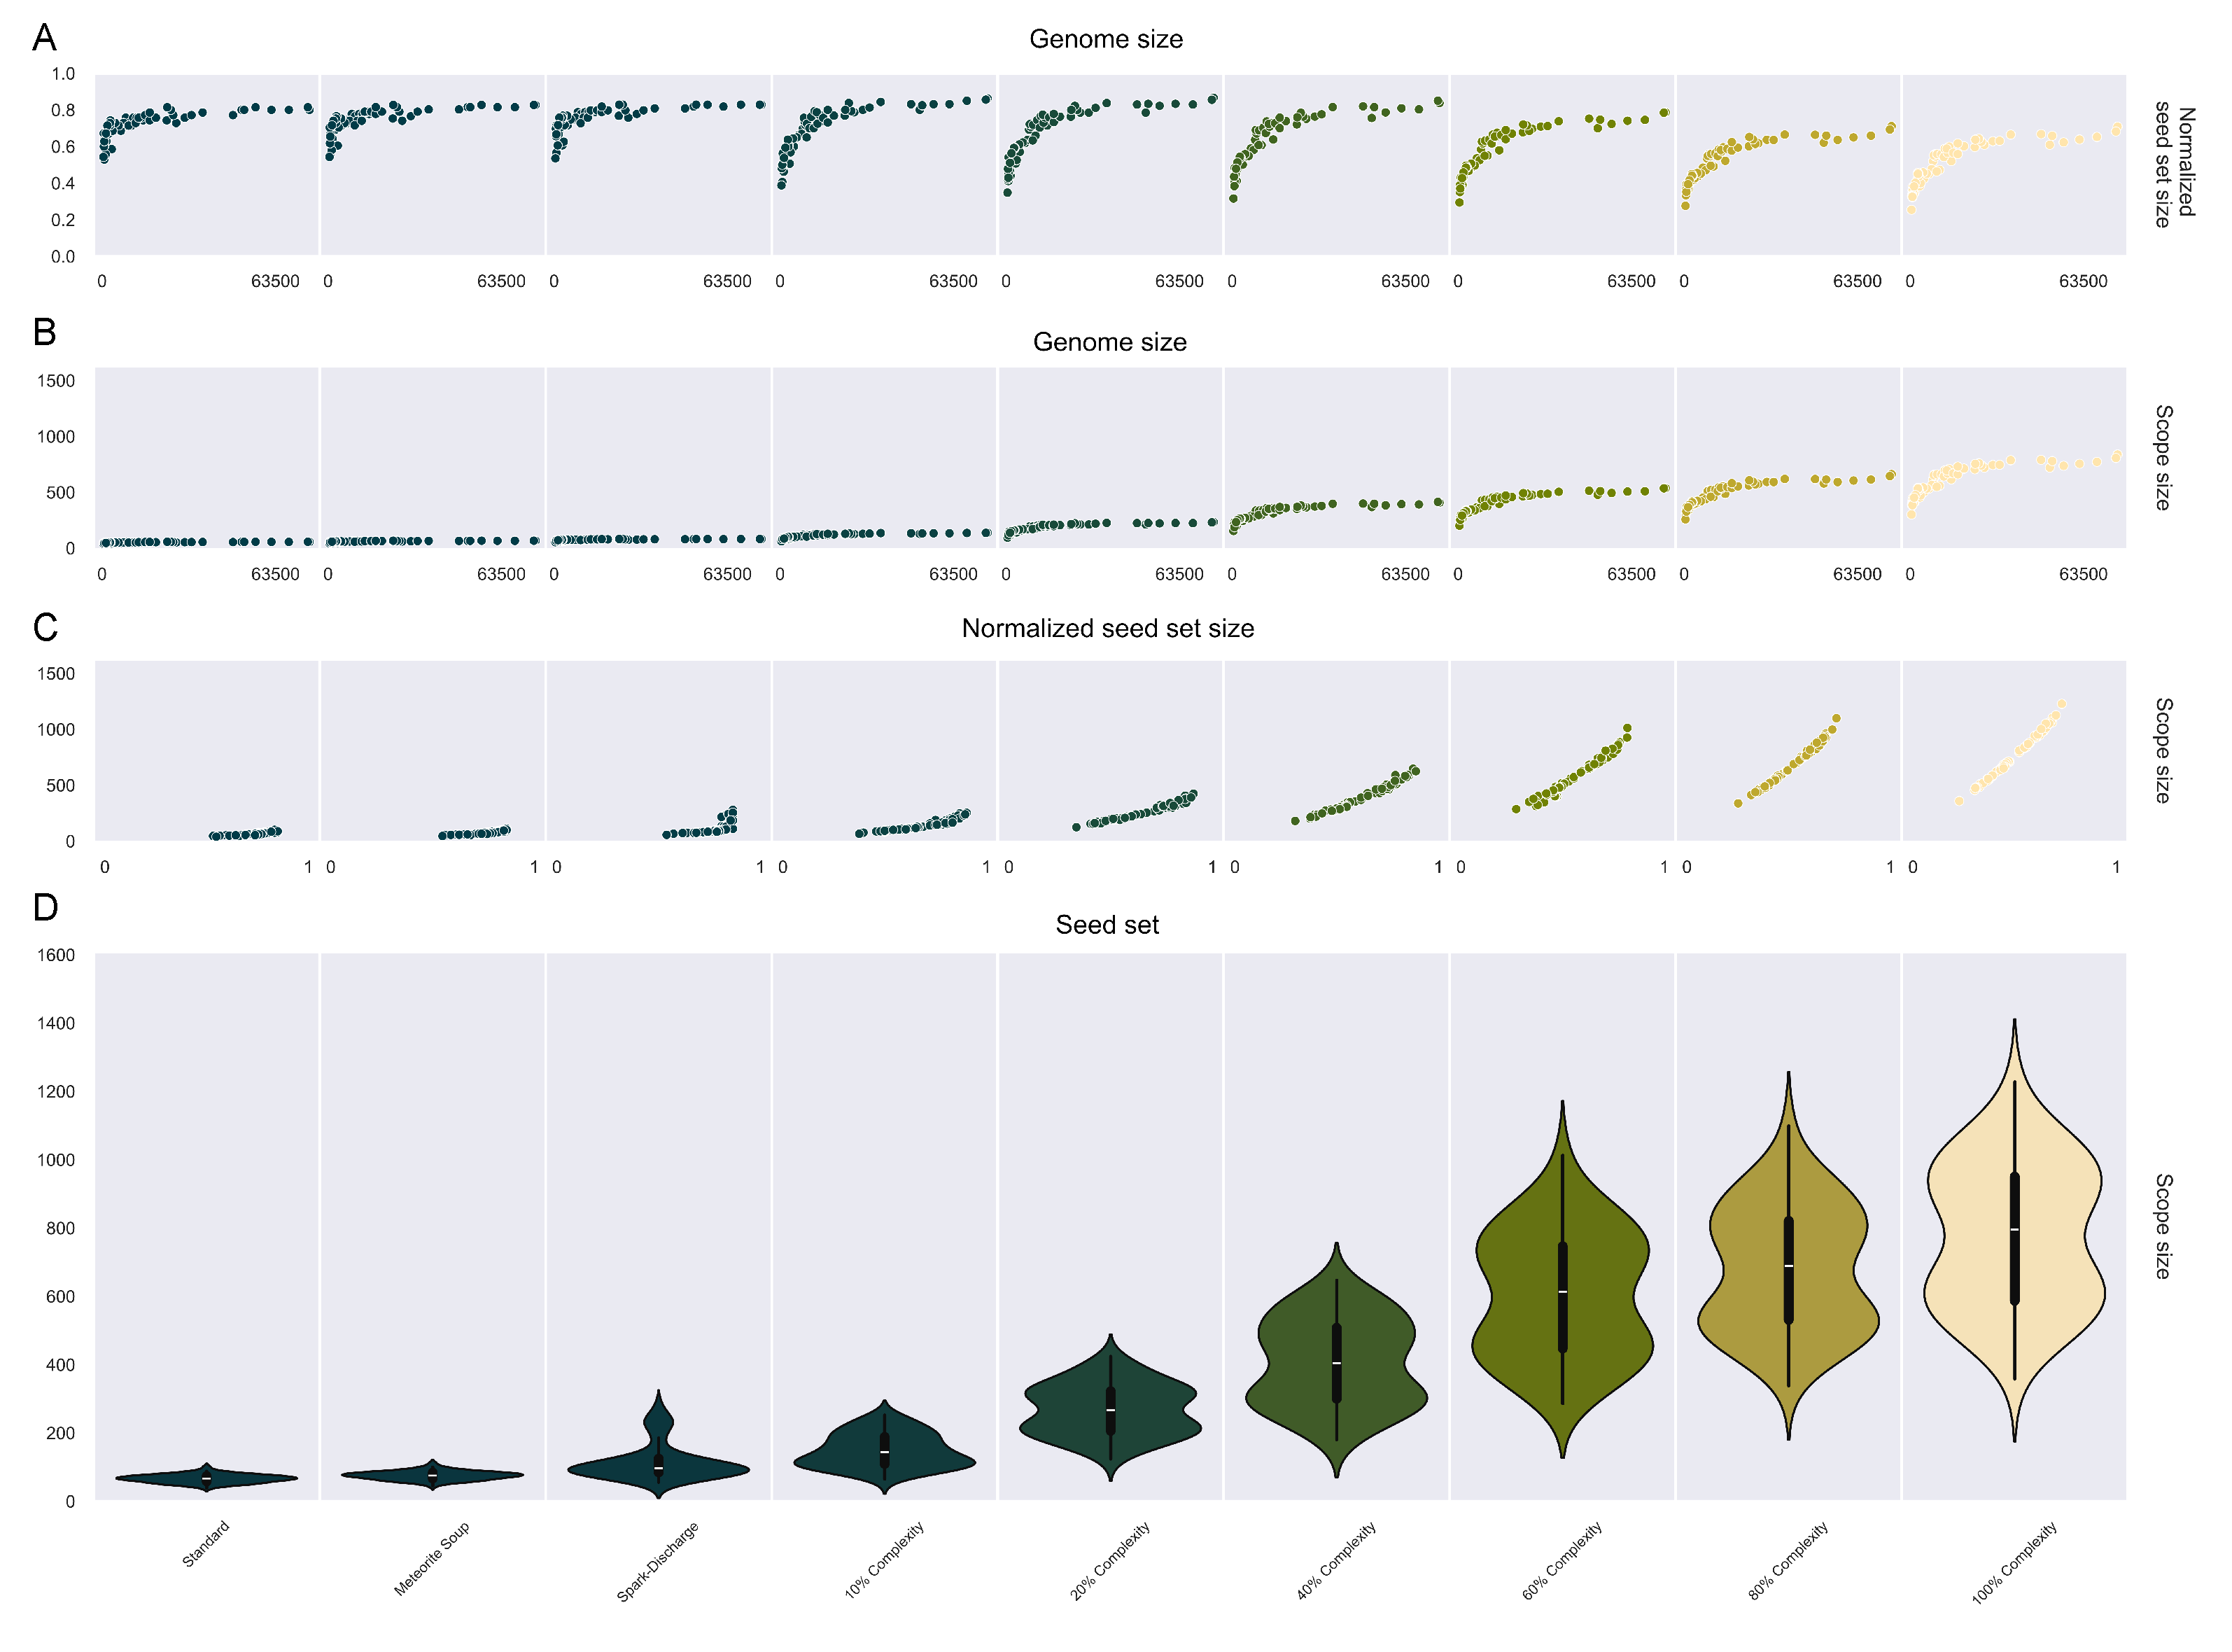
\includegraphics[width=0.98\textwidth]{overview_expansion/overview_ancient_final.pdf}
    \caption{}
    \label{overview_ancient}
\end{figure}   


\begin{figure}[H]
    \centering
    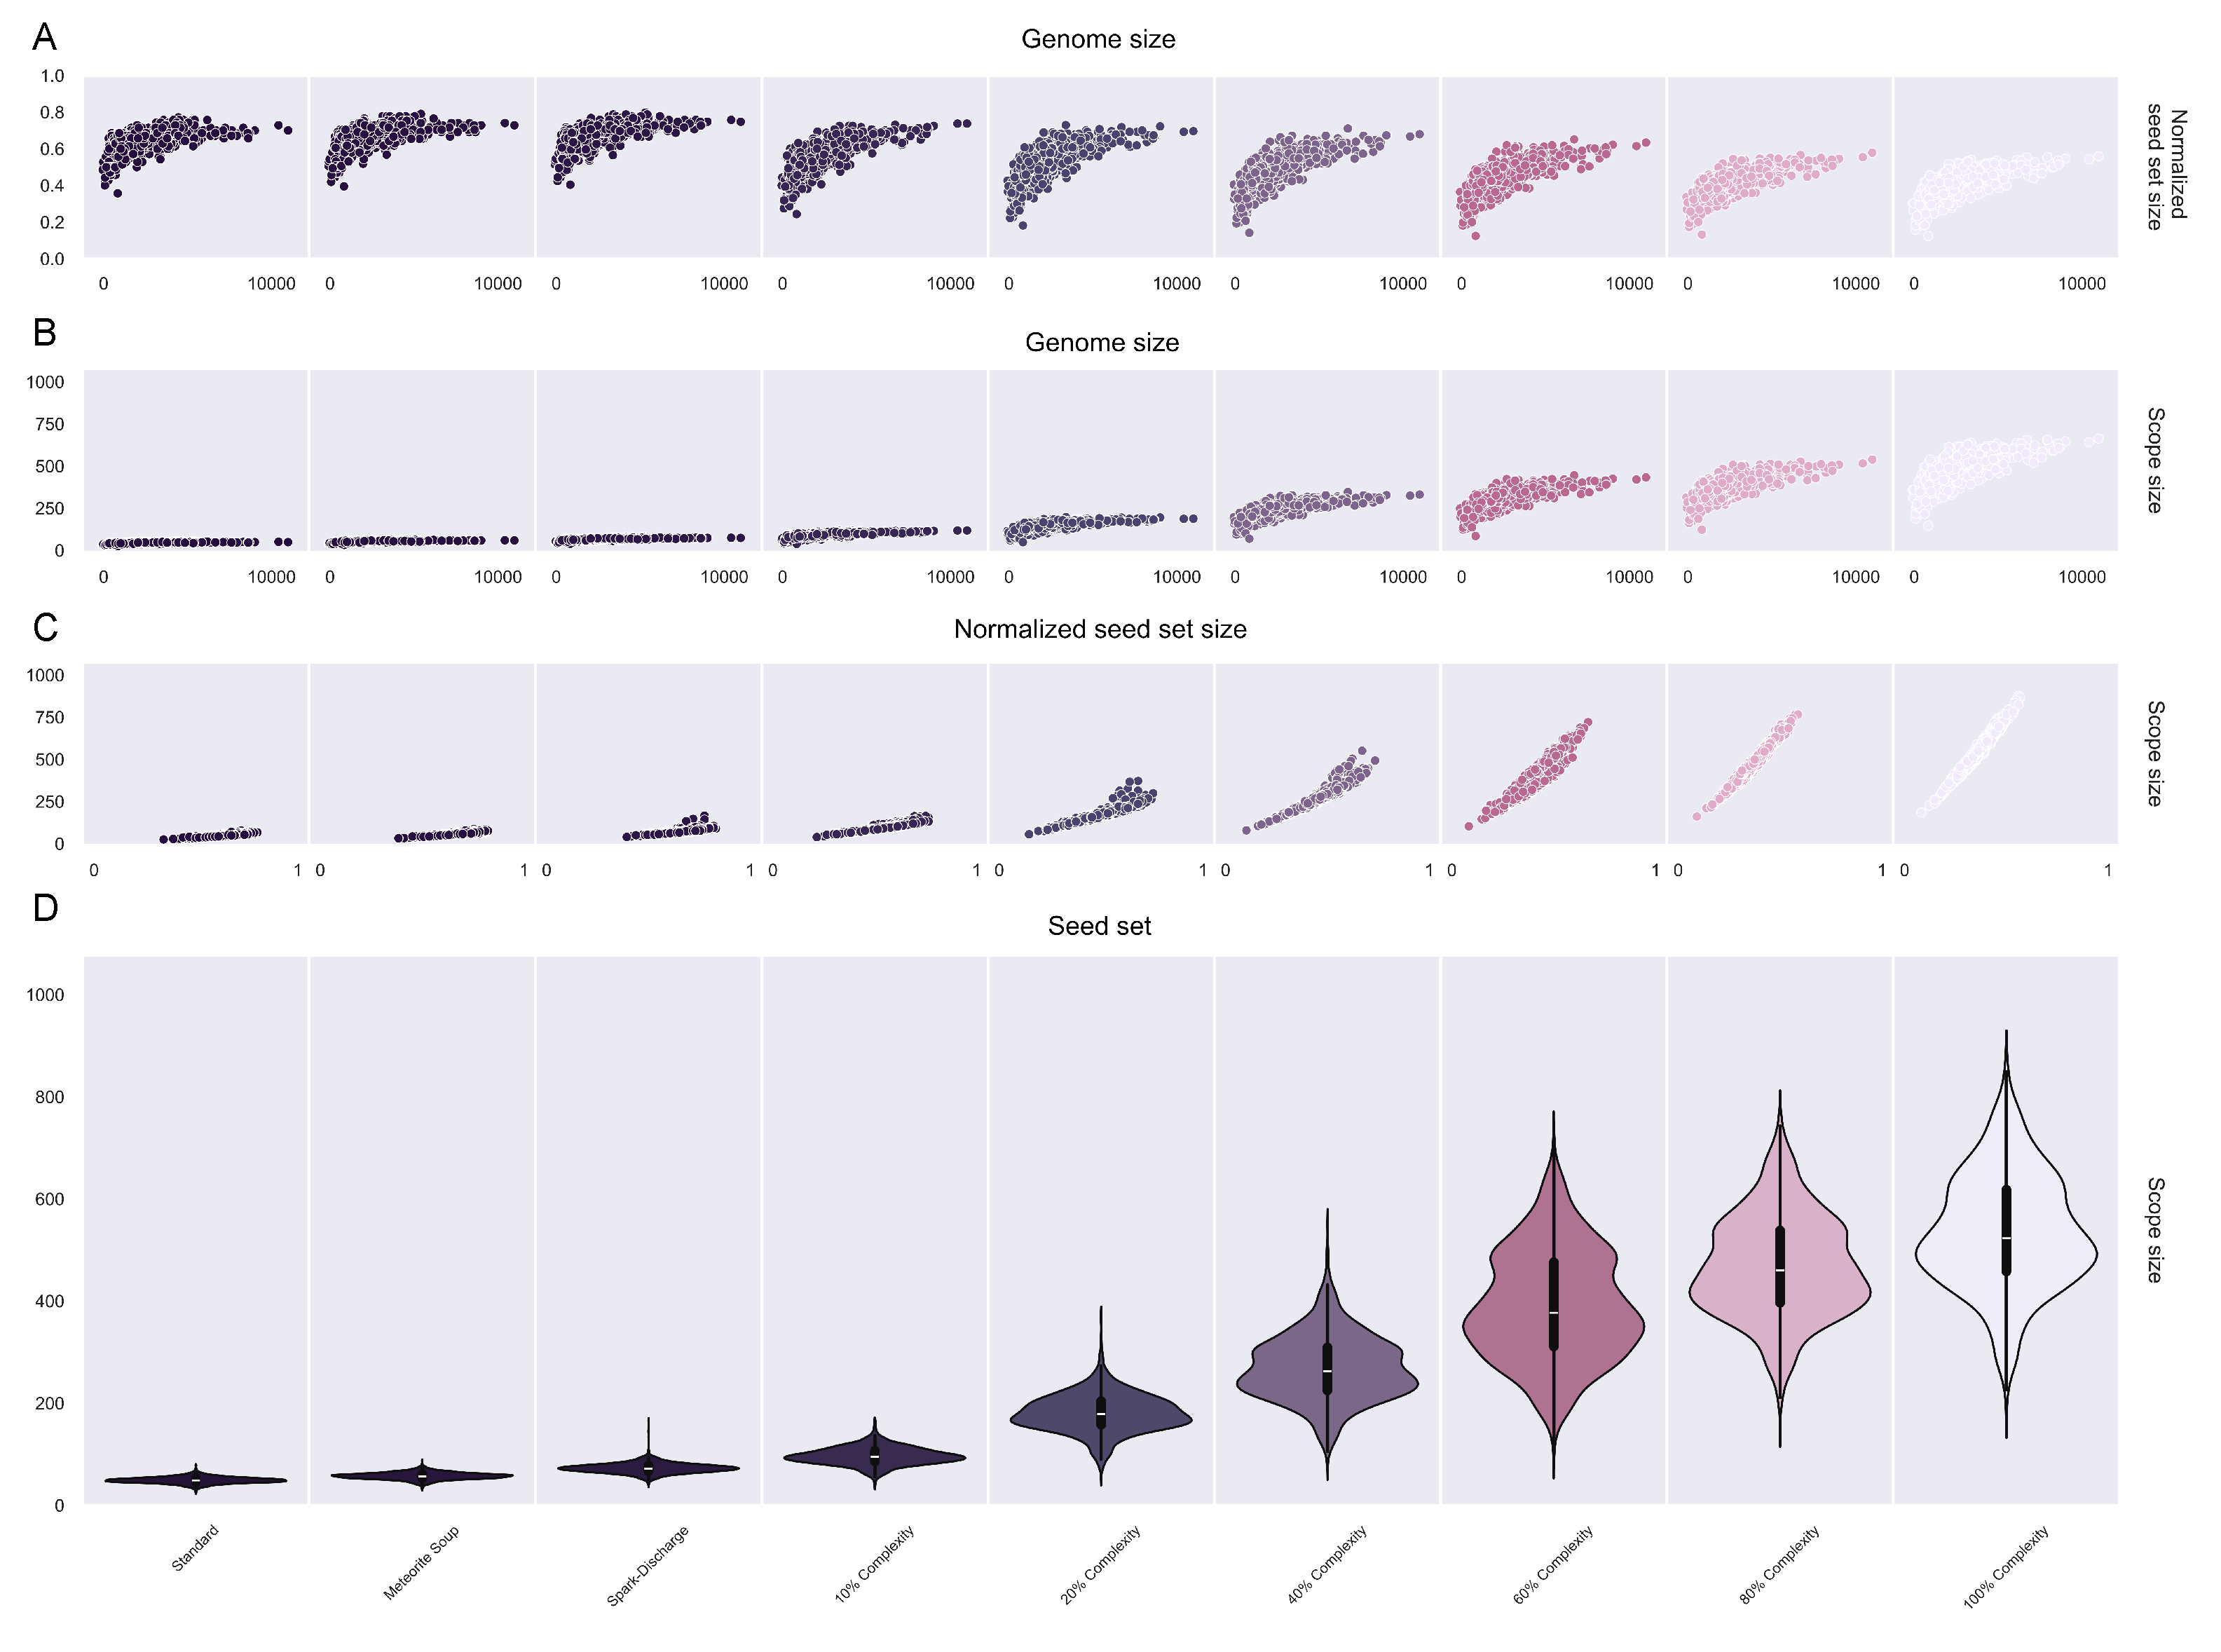
\includegraphics[width=0.98\textwidth]{overview_expansion/overview_extant_final.pdf}
    \caption{}
    \label{overview_extant}
\end{figure}   

\begin{figure}[H]
    \centering
    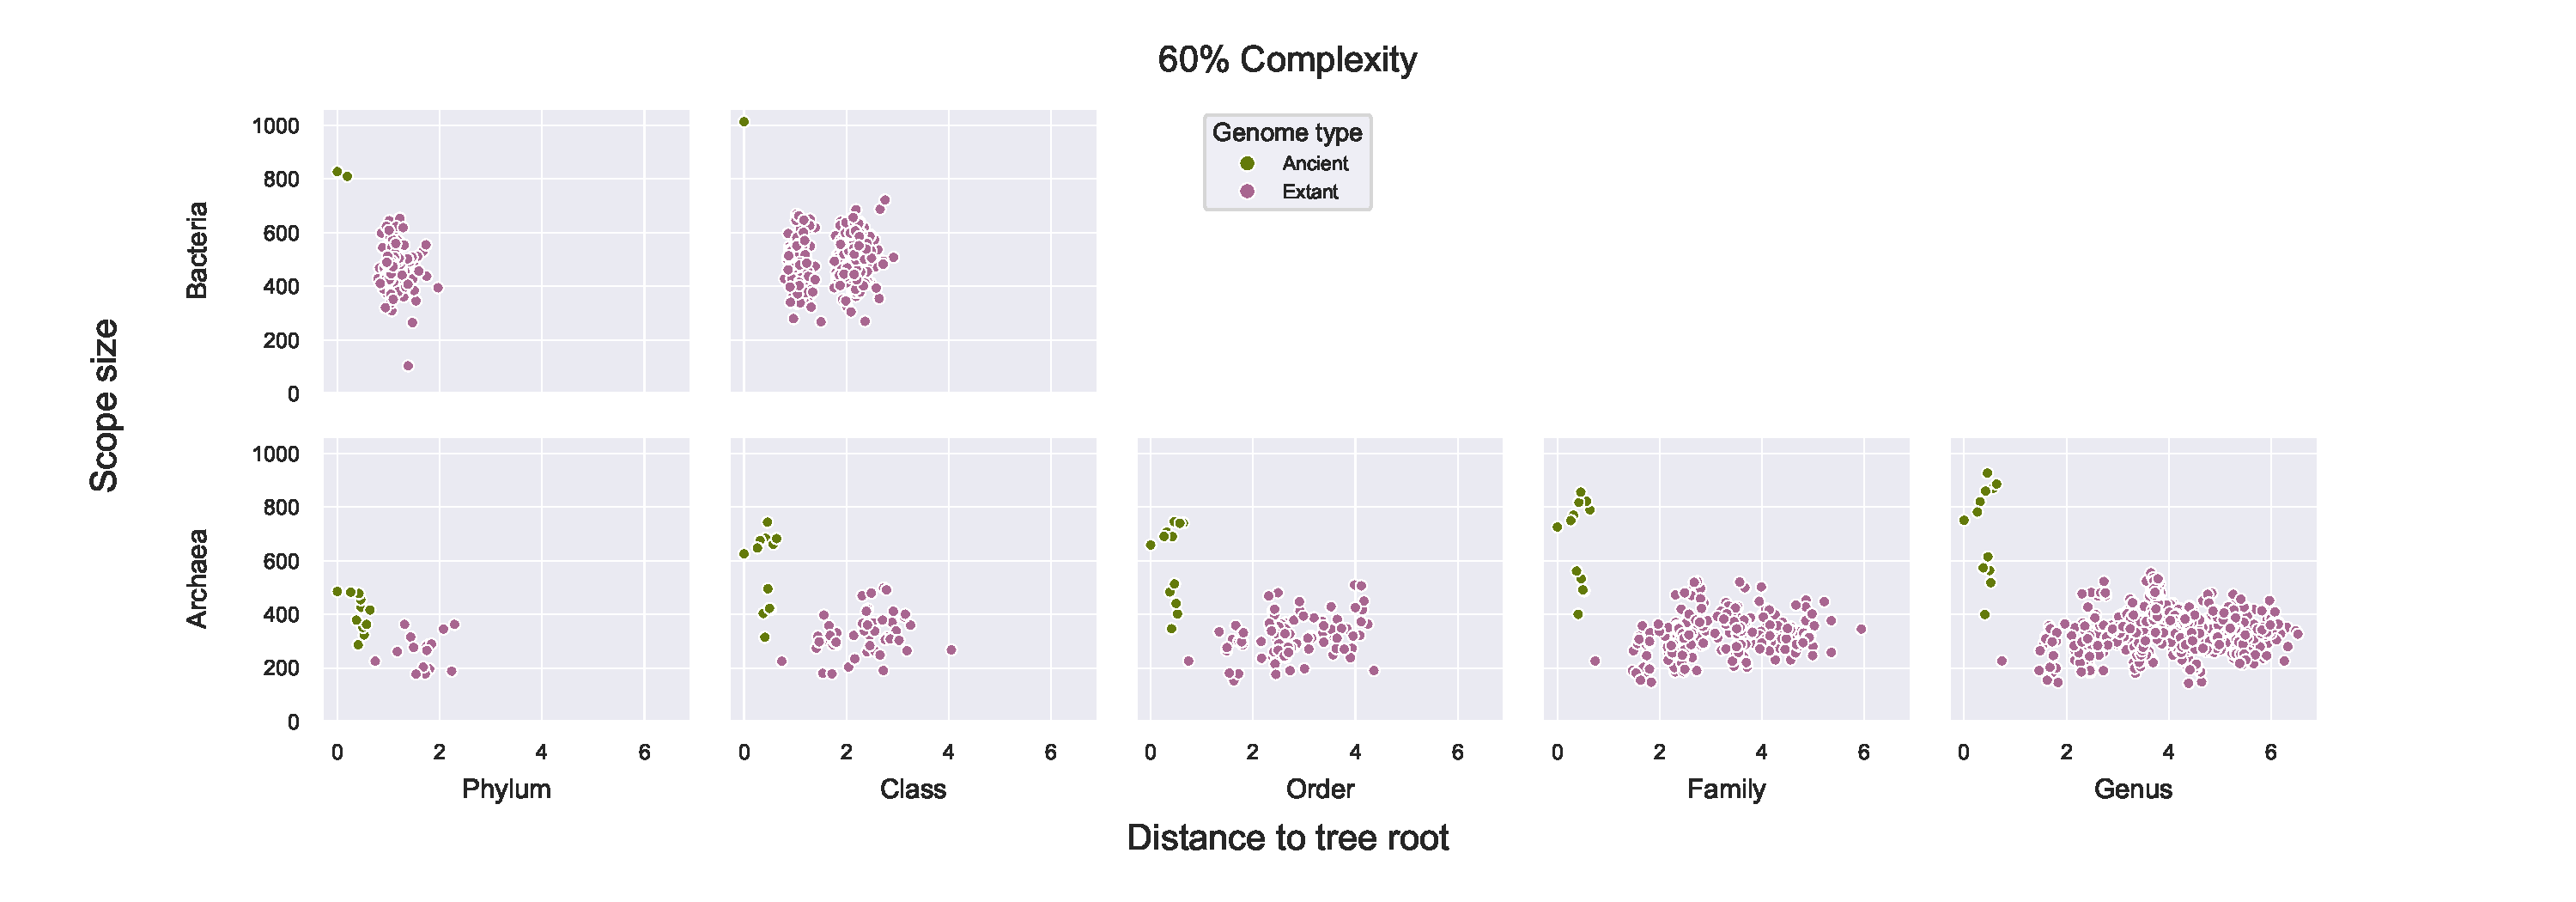
\includegraphics[width=0.95\textwidth]{scopesize_vs_disttoroot/0.6_ss_rootdist.pdf}
    \caption{}
    \label{0.6_scopesize}
\end{figure}   

\begin{figure}[H]
    \centering
    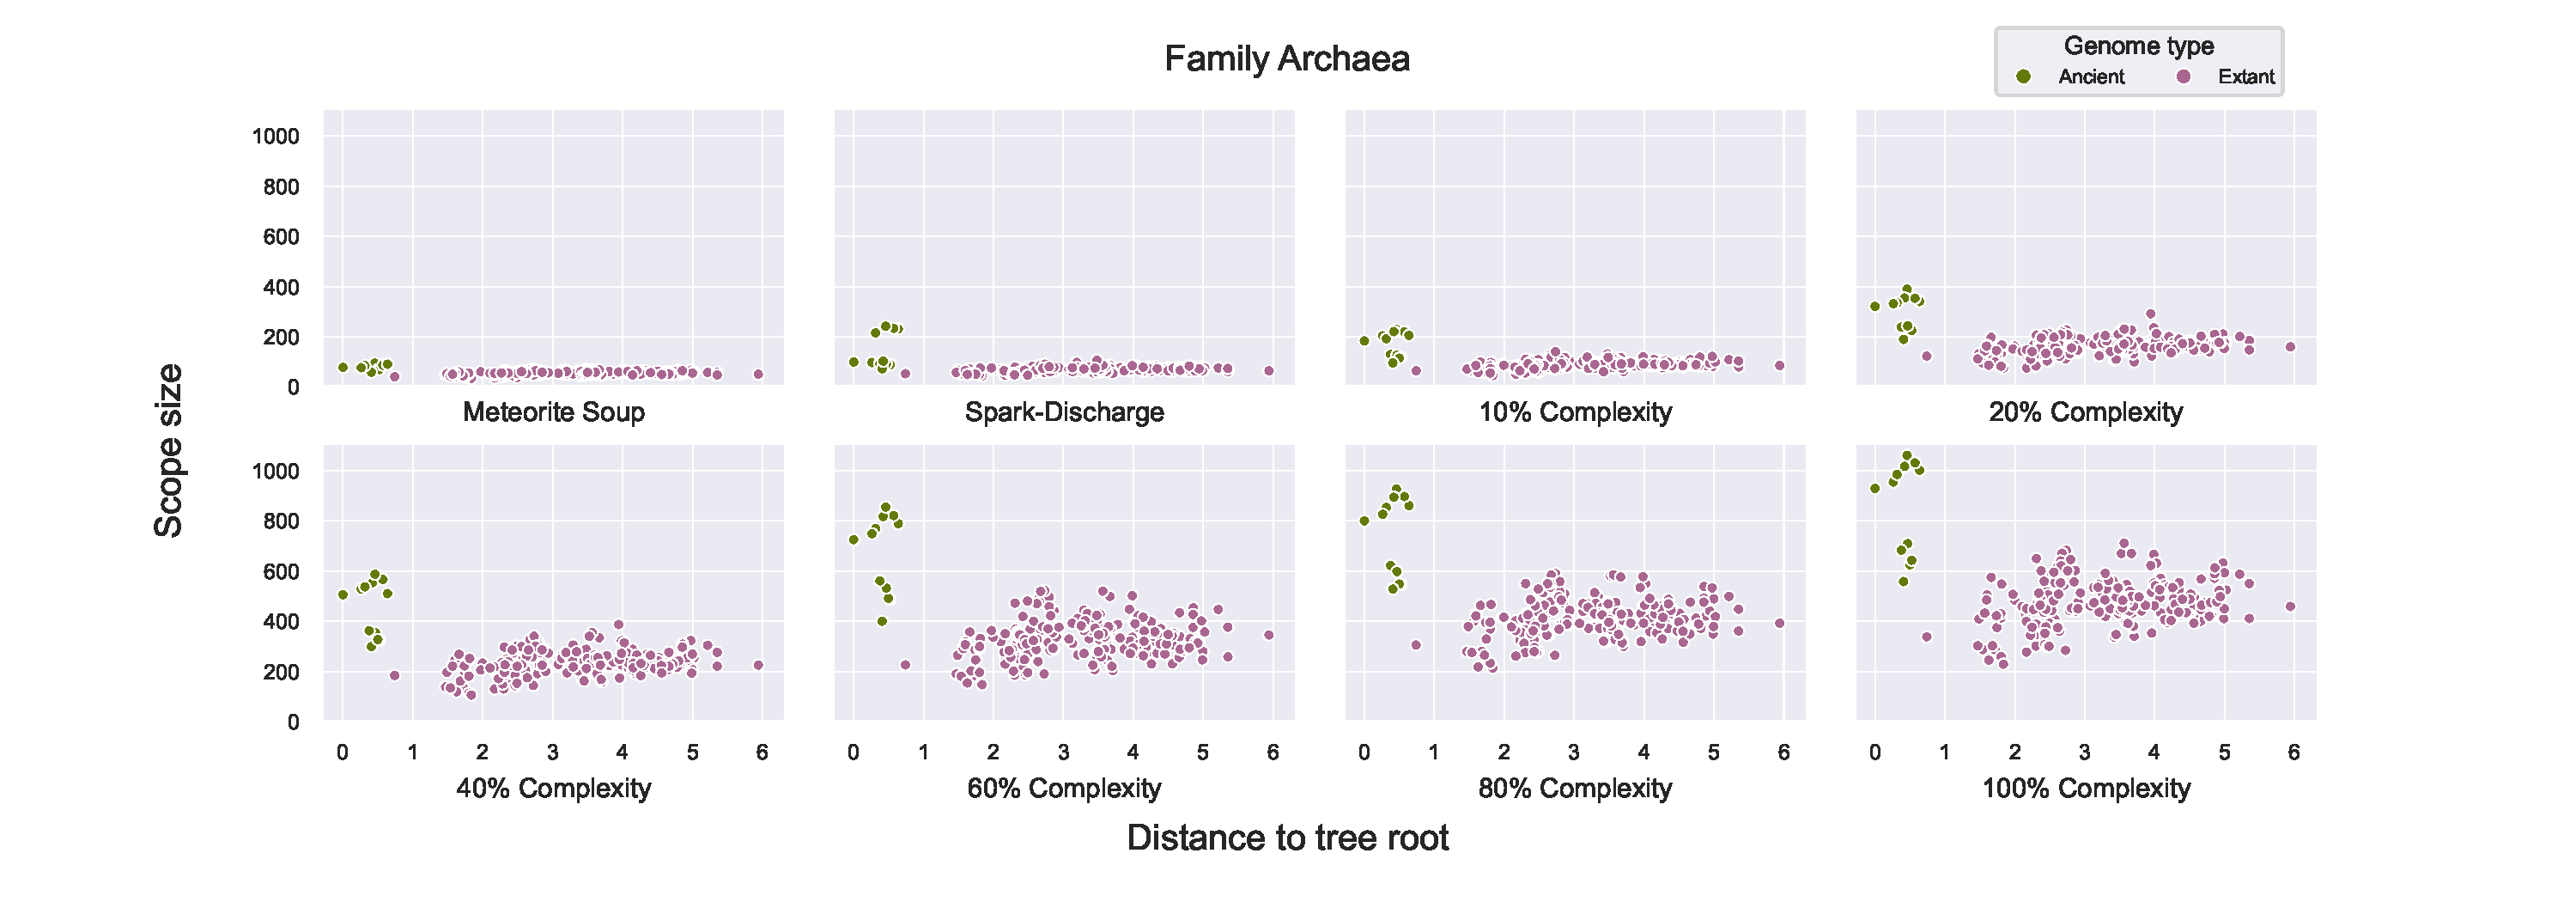
\includegraphics[width=0.95\textwidth]{scopesize_vs_disttoroot/fam4arc_ss_rootdist.pdf}
    \caption{}
    \label{fam_scopesize}
\end{figure}   



\begin{itemize}
    \item For inferred ancient genomes. Explaining main figure.
        \item Network patchiness (not all seeds being present in network, view iterations, low expansion)
        \item Maybe a figure to present patchiness of an N0 network? See how well seeds are "represented" there 
    \item Additional figure: EC values vs root distance (how it changes)
    \item For extant genomes. Explaining main figure.
\end{itemize}